\section{Overview and Motivation (Problem Formulation)}\label{sec:c3s1}
\kant[6-11]

This section builds on the material in \cref{ch:3}, \cref{ch:4} and the prior work of \citet{ch3-4}; see also \citep{ch3-14,ch3-9}.

\begin{equation}\label{eq:c3s1-a}
  I = \int_{0}^{1}\!\!\int_{0}^{1} \frac{\sin(\pi x)\sin(\pi y)}{1+x^2+y^2}\,\mathrm{d}x\,\mathrm{d}y \approx \frac{1}{M}\sum_{m=1}^{M} h(\xi_m),
\end{equation}
with variance decreasing as
\begin{equation}\label{eq:c3s1-b}
  \operatorname{Var}\bigl[\hat I_M\bigr] = \frac{1}{M}\Bigl(\int h^2\,\mathrm{d}\mu - I^2\Bigr) = \mathcal{O}(M^{-1}).
\end{equation}

Equations~\eqref{eq:c3s1-a} and~\eqref{eq:c3s1-b} are used throughout the remainder of this section.

\lipsum[72-73]

\subsection{Quantitative behaviour}\label{sec:c3s1-q}
Results are collected in \cref{tab:c3s1} and visualised in \cref{fig:c3s1-f1}. Similar trends were reported in~\citep{ch3-5,ch3-7}.

\begin{table}[htbp]
\centering
\caption{Summary of measured quantities for experiment set \texttt{c3s1}.}\label{tab:c3s1}
\begin{tabular}{lrrr}
\toprule
Method & Score & Latency & Error \\
\midrule
Alpha & \num{1.7} & \SI{8.46}{\milli\second} & \num{1.227e-3} \\
Beta & \num{4.3} & \SI{4.78}{\milli\second} & \num{7.517e-2} \\
Gamma & \num{36.5} & \SI{6.14}{\milli\second} & \num{3.938e-2} \\
Delta & \num{79.2} & \SI{7.55}{\milli\second} & \num{4.505e-2} \\
Epsilon & \num{49.1} & \SI{0.23}{\milli\second} & \num{1.485e-1} \\
\bottomrule
\end{tabular}
\end{table}

\begin{figure}[htbp]
\centering
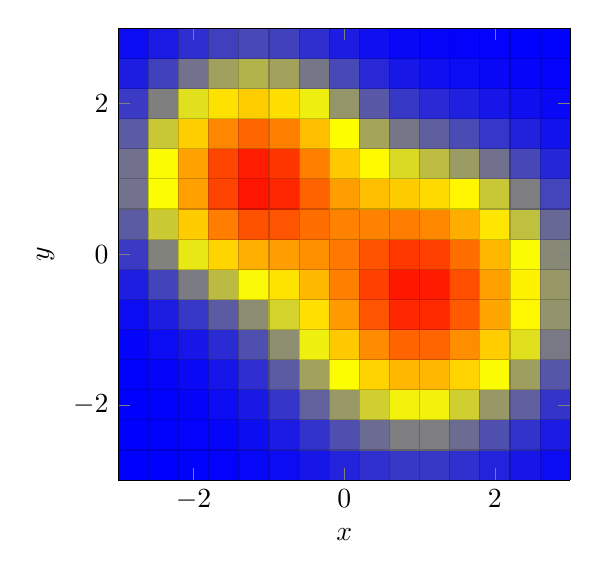
\begin{tikzpicture}\begin{axis}[width=0.7\linewidth,view={0}{90},colormap/hot,xlabel=$x$,ylabel=$y$,axis equal image]
\addplot3[surf,samples=16,domain=-3:3]{exp(-((x-1)^2+(y+0.5)^2)/2.0)+exp(-((x+1.2)^2+(y-1)^2)/1.3333333333333333)};
\end{axis}\end{tikzpicture}
\caption{Generated figure for \texttt{c3s1-f1} (parameters $a=2$, $b=4$).}\label{fig:c3s1-f1}
\end{figure}

\kant[7-11]

\subsection{Implementation notes}\label{sec:c3s1-i}
The core routine is shown in \cref{lst:c3s1}; its complexity is $\mathcal{O}(N\log N)$ per iteration~\cite{ch3-12}.

\begin{lstlisting}[language=python,caption={Reference implementation for c3s1.},label={lst:c3s1}]
def conjugate_gradient(A, b, tol=1e-8, maxit=500):
    x = b * 0
    r = b - A @ x
    p = r.copy()
    for k in range(maxit):
        Ap = A @ p
        alpha = (r @ r) / (p @ Ap)
        x += alpha * p
        r_new = r - alpha * Ap
        if (r_new @ r_new) ** 0.5 < tol:
            break
        p = r_new + ((r_new @ r_new) / (r @ r)) * p
        r = r_new
    return x
\end{lstlisting}

\kant[6-10]
\begin{theorem}\label{thm:c3s1}
Let $A\in\mathbb{R}^{n\times n}$ be symmetric positive definite with condition number $\kappa$. Then the iteration converges and
$\lVert e_k\rVert_A \le 2\bigl(\tfrac{\sqrt\kappa-1}{\sqrt\kappa+1}\bigr)^k\lVert e_0\rVert_A$.
\end{theorem}
\begin{enumerate}[label=(\roman*)]
\item the bound in \cref{thm:c3s1} is sharp for some initial errors;
\item the constant $2$ cannot be improved in general;
\item preconditioning reduces the effective $\kappa$.
\end{enumerate}

\begin{figure}[htbp]
\centering
\includegraphics[width=0.45\linewidth]{stripes.png}
\caption{Raster/vector asset \texttt{stripes.png} included from the figures directory.}\label{fig:c3s1-i0}
\end{figure}

\kant[9-10]
